\chapter{Électronique}

\section{La lumière : Shield LDR}
\subsection{Schéma du Shield LDR}
\begin{figure}[H]
	\centering
	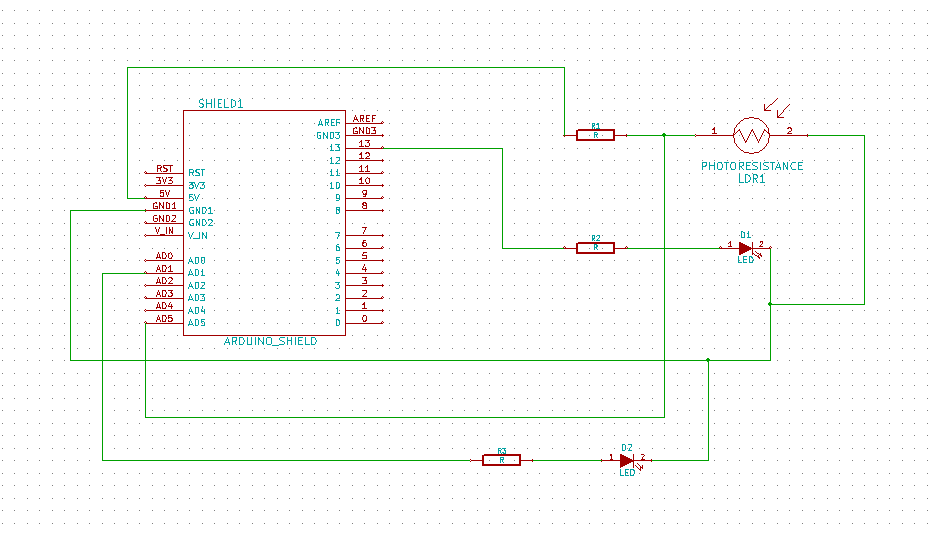
\includegraphics[width=550px]{images/SchemaElectriqueShield.png}
	\caption{Logiciel utilisé : Eeschema de Kicad}
\end{figure}

\subsection{Choix des composants} 
	Notre projet étant une reprise d'un projet de l'année dernière, nous avons dû refaire le shield. Nous avons donc récupéré leurs composants à savoir :
	\begin{itemize}
		\item Une Arduino Mega 2560
		\item Deux LEDs 
		\item Une photorésistance LDR
		\item Trois résistances
	\end{itemize}

\section{Alimentation autonome : 7805}
\subsection{Schéma du régulateur de tension}
\begin{figure}[H]
	\centering
	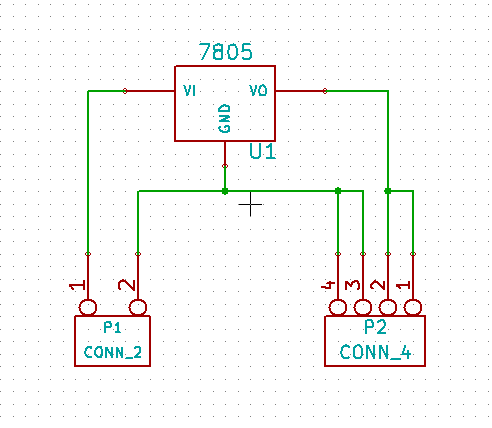
\includegraphics[width=350px]{images/SchemaDuRegulateur.png}
	\caption{Logiciel utilisé : Eeschema de Kicad}
\end{figure}

\subsection{Choix des composants} 
	Nos camarades de l'année dernière alimentaient leurs Arduino et Raspberry avec une prise secteur. Cette année, nous avons décidé d'en faire un réveil portable. Et qui dit portable, dit alimentation autonome. Les deux appareils étant alimentés en 5V, nous avons commandé un régulateur de tension 7805 qui délivre du 5V/1A. On met donc en entrée du régulateur un pack d'accus de 7V et le régulateur va se charger de délivrer du 5V à l'Arduino et à la Raspberry branchées en dérivation sur celui-ci.

\section{Communication Arduino-Raspberry}
	Comme la Arduino reçoit les informations du capteur de luminosité et allume la lampe, et que le Raspberry est en charge du réveil, il a fallu établir une communication entre les deux cartes. Pour cela nous utilisons deux pins du Raspberry et deux pins du la Arduino afin de pouvoir envoyer et recevoir des informations grâce à une liaison bi-directionnelle.\\

	D'un côté, le Raspberry va envoyer un signal de réveil à la Arduino afin qu'elle puisse commencer à allumer la LED. Et inversement, lorsque que la Arduino détecte une source de lumière, elle envoie un signal au Raspberry afin qu'il puisse éteindre la sonnerie du réveil.